\documentclass{standalone}
\usepackage{tikz}
\usetikzlibrary{patterns, positioning}

\begin{document}
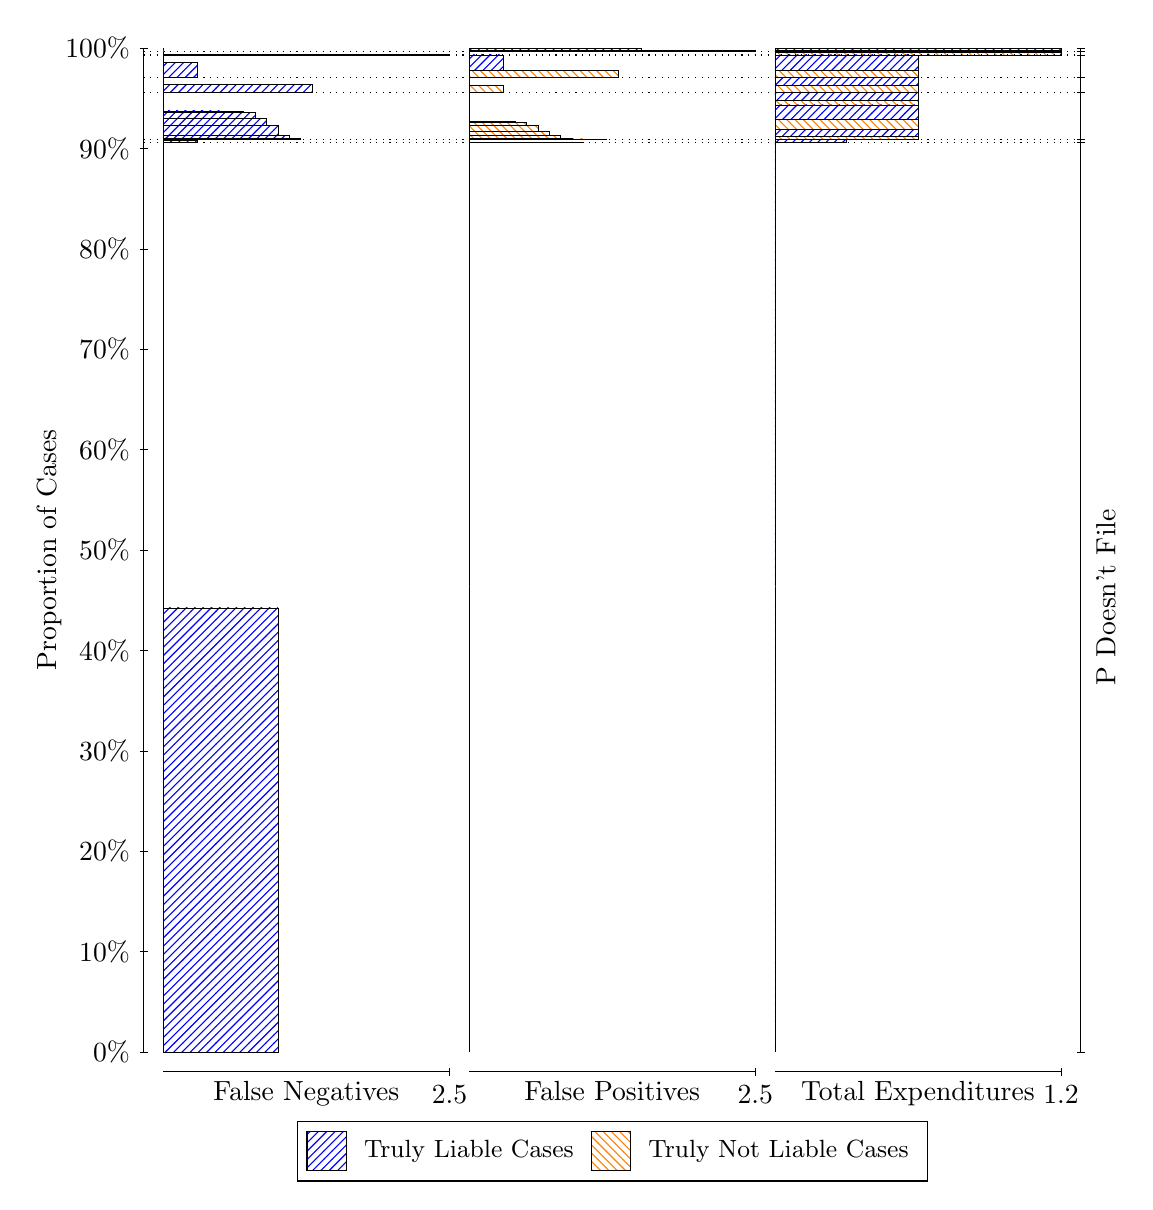
\begin{tikzpicture}
\draw[black, very thin] (1.5,1.75) -- (1.5,14.5);
\node[rotate=90, anchor=center] at (0.3, 8.125) {Proportion of Cases};
\draw[black, very thin] (1.45,1.75) -- (1.55,1.75);
\node[anchor=east] at (1.45, 1.75) {0\%};
\draw[black, very thin] (1.45,3.025) -- (1.55,3.025);
\node[anchor=east] at (1.45, 3.025) {10\%};
\draw[black, very thin] (1.45,4.3) -- (1.55,4.3);
\node[anchor=east] at (1.45, 4.3) {20\%};
\draw[black, very thin] (1.45,5.575) -- (1.55,5.575);
\node[anchor=east] at (1.45, 5.575) {30\%};
\draw[black, very thin] (1.45,6.85) -- (1.55,6.85);
\node[anchor=east] at (1.45, 6.85) {40\%};
\draw[black, very thin] (1.45,8.125) -- (1.55,8.125);
\node[anchor=east] at (1.45, 8.125) {50\%};
\draw[black, very thin] (1.45,9.4) -- (1.55,9.4);
\node[anchor=east] at (1.45, 9.4) {60\%};
\draw[black, very thin] (1.45,10.675) -- (1.55,10.675);
\node[anchor=east] at (1.45, 10.675) {70\%};
\draw[black, very thin] (1.45,11.95) -- (1.55,11.95);
\node[anchor=east] at (1.45, 11.95) {80\%};
\draw[black, very thin] (1.45,13.225) -- (1.55,13.225);
\node[anchor=east] at (1.45, 13.225) {90\%};
\draw[black, very thin] (1.45,14.5) -- (1.55,14.5);
\node[anchor=east] at (1.45, 14.5) {100\%};

\draw[black, very thin] (13.4,1.75) -- (13.4,14.5);
\draw[black, very thin] (13.35,1.75) -- (13.45,1.75);
\node[anchor=west] at (13.35, 1.75) {};
\draw[black, very thin] (13.35,13.302) -- (13.45,13.302);
\node[anchor=west] at (13.35, 13.302) {};
\draw[black, very thin] (13.35,13.337) -- (13.45,13.337);
\node[anchor=west] at (13.35, 13.337) {};
\draw[black, very thin] (13.35,13.933) -- (13.45,13.933);
\node[anchor=west] at (13.35, 13.933) {};
\draw[black, very thin] (13.35,14.125) -- (13.45,14.125);
\node[anchor=west] at (13.35, 14.125) {};
\draw[black, very thin] (13.35,14.412) -- (13.45,14.412);
\node[anchor=west] at (13.35, 14.412) {};
\draw[black, very thin] (13.35,14.459) -- (13.45,14.459);
\node[anchor=west] at (13.35, 14.459) {};
\draw[black, very thin] (13.35,14.5) -- (13.45,14.5);
\node[anchor=west] at (13.35, 14.5) {};

\draw[black, very thin, pattern color=blue, pattern=north east lines] (1.75,1.75) rectangle (3.2033,7.3907);
\draw[black, very thin, pattern color=orange, pattern=north west lines] (1.75,7.3907) rectangle (1.75,13.302);
\draw[black, very thin, pattern color=blue, pattern=north east lines] (1.75,13.302) rectangle (2.186,13.333);
\draw[black, very thin, pattern color=orange, pattern=north west lines] (1.75,13.333) rectangle (1.75,13.337);
\draw[black, very thin, pattern color=blue, pattern=north east lines] (1.75,13.337) rectangle (3.494,13.35);
\draw[black, very thin, pattern color=blue, pattern=north east lines] (1.75,13.35) rectangle (3.3487,13.391);
\draw[black, very thin, pattern color=blue, pattern=north east lines] (1.75,13.391) rectangle (3.2033,13.515);
\draw[black, very thin, pattern color=blue, pattern=north east lines] (1.75,13.515) rectangle (3.058,13.517);
\draw[black, very thin, pattern color=blue, pattern=north east lines] (1.75,13.517) rectangle (3.058,13.608);
\draw[black, very thin, pattern color=blue, pattern=north east lines] (1.75,13.608) rectangle (2.9127,13.687);
\draw[black, very thin, pattern color=blue, pattern=north east lines] (1.75,13.687) rectangle (2.7673,13.693);
\draw[black, very thin, pattern color=blue, pattern=north east lines] (1.75,13.693) rectangle (2.622,13.698);
\draw[black, very thin, pattern color=blue, pattern=north east lines] (1.75,13.698) rectangle (2.4767,13.701);
\draw[black, very thin, pattern color=blue, pattern=north east lines] (1.75,13.701) rectangle (2.3313,13.703);
\draw[black, very thin, pattern color=orange, pattern=north west lines] (1.75,13.703) rectangle (1.75,13.933);
\draw[black, very thin, pattern color=blue, pattern=north east lines] (1.75,13.933) rectangle (3.6393,14.035);
\draw[black, very thin, pattern color=orange, pattern=north west lines] (1.75,14.035) rectangle (1.75,14.125);
\draw[black, very thin, pattern color=blue, pattern=north east lines] (1.75,14.125) rectangle (2.186,14.319);
\draw[black, very thin, pattern color=orange, pattern=north west lines] (1.75,14.319) rectangle (1.75,14.412);
\draw[black, very thin, pattern color=blue, pattern=north east lines] (1.75,14.412) rectangle (5.3833,14.421);
\draw[black, very thin, pattern color=orange, pattern=north west lines] (1.75,14.421) rectangle (1.75,14.459);
\draw[black, very thin, pattern color=orange, pattern=north west lines] (1.75,14.459) rectangle (1.75,14.468);
\draw[black, very thin, pattern color=blue, pattern=north east lines] (1.75,14.468) rectangle (1.75,14.5);
\draw[black, very thin, pattern color=orange, pattern=north west lines] (5.6333,1.75) rectangle (5.6333,7.661);
\draw[black, very thin, pattern color=blue, pattern=north east lines] (5.6333,7.661) rectangle (5.6333,13.302);
\draw[black, very thin, pattern color=orange, pattern=north west lines] (5.6333,13.302) rectangle (7.0867,13.306);
\draw[black, very thin, pattern color=blue, pattern=north east lines] (5.6333,13.306) rectangle (5.6333,13.337);
\draw[black, very thin, pattern color=orange, pattern=north west lines] (5.6333,13.337) rectangle (7.3773,13.34);
\draw[black, very thin, pattern color=orange, pattern=north west lines] (5.6333,13.34) rectangle (7.232,13.342);
\draw[black, very thin, pattern color=orange, pattern=north west lines] (5.6333,13.342) rectangle (7.0867,13.346);
\draw[black, very thin, pattern color=orange, pattern=north west lines] (5.6333,13.346) rectangle (6.9413,13.351);
\draw[black, very thin, pattern color=orange, pattern=north west lines] (5.6333,13.351) rectangle (6.796,13.39);
\draw[black, very thin, pattern color=orange, pattern=north west lines] (5.6333,13.39) rectangle (6.6507,13.441);
\draw[black, very thin, pattern color=orange, pattern=north west lines] (5.6333,13.441) rectangle (6.5053,13.521);
\draw[black, very thin, pattern color=orange, pattern=north west lines] (5.6333,13.521) rectangle (6.36,13.552);
\draw[black, very thin, pattern color=orange, pattern=north west lines] (5.6333,13.552) rectangle (6.2147,13.567);
\draw[black, very thin, pattern color=blue, pattern=north east lines] (5.6333,13.567) rectangle (5.924,13.57);
\draw[black, very thin, pattern color=blue, pattern=north east lines] (5.6333,13.57) rectangle (5.7787,13.572);
\draw[black, very thin, pattern color=blue, pattern=north east lines] (5.6333,13.572) rectangle (5.6333,13.933);
\draw[black, very thin, pattern color=orange, pattern=north west lines] (5.6333,13.933) rectangle (6.0693,14.023);
\draw[black, very thin, pattern color=blue, pattern=north east lines] (5.6333,14.023) rectangle (5.6333,14.125);
\draw[black, very thin, pattern color=orange, pattern=north west lines] (5.6333,14.125) rectangle (7.5227,14.217);
\draw[black, very thin, pattern color=blue, pattern=north east lines] (5.6333,14.217) rectangle (6.0693,14.412);
\draw[black, very thin, pattern color=orange, pattern=north west lines] (5.6333,14.412) rectangle (5.6333,14.45);
\draw[black, very thin, pattern color=blue, pattern=north east lines] (5.6333,14.45) rectangle (5.6333,14.459);
\draw[black, very thin, pattern color=orange, pattern=north west lines] (5.6333,14.459) rectangle (9.2667,14.468);
\draw[black, very thin, pattern color=blue, pattern=north east lines] (5.6333,14.468) rectangle (7.8133,14.5);
\draw[black, very thin, pattern color=orange, pattern=north west lines] (9.5167,1.75) rectangle (9.5167,7.661);
\draw[black, very thin, pattern color=blue, pattern=north east lines] (9.5167,7.661) rectangle (9.5167,13.302);
\draw[black, very thin, pattern color=orange, pattern=north west lines] (9.5167,13.302) rectangle (10.425,13.306);
\draw[black, very thin, pattern color=blue, pattern=north east lines] (9.5167,13.306) rectangle (10.425,13.337);
\draw[black, very thin, pattern color=orange, pattern=north west lines] (9.5167,13.337) rectangle (11.333,13.382);
\draw[black, very thin, pattern color=blue, pattern=north east lines] (9.5167,13.382) rectangle (11.333,13.469);
\draw[black, very thin, pattern color=orange, pattern=north west lines] (9.5167,13.469) rectangle (11.333,13.597);
\draw[black, very thin, pattern color=blue, pattern=north east lines] (9.5167,13.597) rectangle (11.333,13.777);
\draw[black, very thin, pattern color=orange, pattern=north west lines] (9.5167,13.777) rectangle (11.333,13.834);
\draw[black, very thin, pattern color=blue, pattern=north east lines] (9.5167,13.834) rectangle (11.333,13.933);
\draw[black, very thin, pattern color=orange, pattern=north west lines] (9.5167,13.933) rectangle (11.333,14.023);
\draw[black, very thin, pattern color=blue, pattern=north east lines] (9.5167,14.023) rectangle (11.333,14.125);
\draw[black, very thin, pattern color=orange, pattern=north west lines] (9.5167,14.125) rectangle (11.333,14.217);
\draw[black, very thin, pattern color=blue, pattern=north east lines] (9.5167,14.217) rectangle (11.333,14.412);
\draw[black, very thin, pattern color=orange, pattern=north west lines] (9.5167,14.412) rectangle (13.15,14.45);
\draw[black, very thin, pattern color=blue, pattern=north east lines] (9.5167,14.45) rectangle (13.15,14.459);
\draw[black, very thin, pattern color=orange, pattern=north west lines] (9.5167,14.459) rectangle (13.15,14.468);
\draw[black, very thin, pattern color=blue, pattern=north east lines] (9.5167,14.468) rectangle (13.15,14.5);
\draw[black, dotted] (1.5,13.302) -- (13.4,13.302);
\draw[black, dotted] (1.5,13.337) -- (13.4,13.337);
\draw[black, dotted] (1.5,13.933) -- (13.4,13.933);
\draw[black, dotted] (1.5,14.125) -- (13.4,14.125);
\draw[black, dotted] (1.5,14.412) -- (13.4,14.412);
\draw[black, dotted] (1.5,14.459) -- (13.4,14.459);
\draw[black, very thin] (1.75,1.5) -- (5.3833,1.5);
\node[anchor=north] at (3.5667, 1.5) {False Negatives};
\draw[black, very thin] (5.3833,1.45) -- (5.3833,1.55);
\node[anchor=north] at (5.3833, 1.45) {2.5};

\draw[black, very thin] (5.6333,1.5) -- (9.2667,1.5);
\node[anchor=north] at (7.45, 1.5) {False Positives};
\draw[black, very thin] (9.2667,1.45) -- (9.2667,1.55);
\node[anchor=north] at (9.2667, 1.45) {2.5};

\draw[black, very thin] (9.5167,1.5) -- (13.15,1.5);
\node[anchor=north] at (11.333, 1.5) {Total Expenditures};
\draw[black, very thin] (13.15,1.45) -- (13.15,1.55);
\node[anchor=north] at (13.15, 1.45) {1.2};

\node[black, centered, rotate=90] at (13.72, 7.5258) {P Doesn't File};







\draw (7.449999999999999,1.5) node[draw=none] (baseCoordinate) {};
\begin{scope}[align=center]
        \matrix[scale=0.5, draw=black, below=0.5cm of baseCoordinate, nodes={draw}, column sep=0.1cm]{
            \node[rectangle, draw, minimum width=0.5cm, minimum height=0.5cm, pattern=north east lines, pattern color=blue] {}; &
            \node[draw=none, font=\small] (B) {Truly Liable Cases}; &
            \node[rectangle, draw, minimum width=0.5cm, minimum height=0.5cm, pattern=north west lines, pattern color=orange] {}; &
            \node[draw=none, font=\small] (B) {Truly Not Liable Cases}; \\
            };
\end{scope}

\end{tikzpicture}
\end{document}